% Toolbar icon: ptMpm — Material point method: particles on a background grid.
% NOTE: the committed svg-ui/ptMpm.svg was generated from this same drawing
% (24-unit grid, 1.6 stroke) without a LaTeX toolchain; regenerating via
% `make ui` replaces it with the pdftocairo rendering of this source — same
% glyph either way.
\documentclass[tikz,border=0pt]{standalone}
\begin{document}
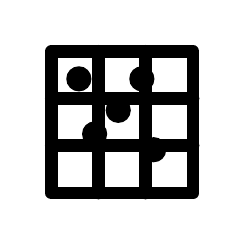
\begin{tikzpicture}[line width=1.6mm, line cap=round, line join=round, x=1mm,y=1mm]
  \useasboundingbox (0,0) rectangle (24,24);
  \draw (3,21) -- (21,21) -- (21,3) -- (3,3) -- cycle;
  \draw (9,21) -- (9,3);
  \draw (15,21) -- (15,3);
  \draw (3,15) -- (21,15);
  \draw (3,9) -- (21,9);
  \fill (6.5,17.5) circle (1.6);
  \fill (11.5,13.5) circle (1.6);
  \fill (8.5,10.5) circle (1.6);
  \fill (16,8.5) circle (1.6);
  \fill (14.5,17.5) circle (1.6);
\end{tikzpicture}
\end{document}
